%!TEX root = ../Thesis.tex


\chapter{Focusing Ultrasound Through An Arbitrary Interface}\label{chap:cuetfm}

\graphicspath{{cueTFM/Images/}}

\section{Theory}
\subsection{Overview}
This chapter introduces a novel approach to dealing with refraction for real time imaging through a refractive interface. This chapter introduces a novel approach to dealing with refraction for real time imaging through a refractive interface. The methodologies and results in this chapter were developed by a research team within the Centre for Ultrasonic Engineering and the University of Strathclyde. This work builds upon the original research performed by Dziewierz\cite{dziewierz_2d_2015} and was subsequently extended by McGilp\cite{mcgilp_adaptation_2016} to produce the results presented in Section \ref{sec:ail_result}.

In industry, inspection of welds is often hampered by their complex geometries. A simple solution to this is to use an array on a conformable wedge\cite{russell_development_2010}. Calculating wave propagation times through an irregular interface is an iterative process and can take a significant amount of time to complete for a real-time interactive implementation of TFM. A new method for interpolation of time delays is presented where the entire imaging algorithm is implemented in Compute Unified Device Architecture (CUDA) C++ and iterative processes are minimised through a curve fitting procedure. In this chapter, an implementation of the TFM algorithm that allows rapid, low-latency imaging through an arbitrary 3D curved refracting interface is presented. 

\subsection{Introduction}

The use of arrays in ultrasonic non-destructive evaluation has opened a door to the application of many different diagnostic methods. Phased arrays can be used to change the effective aperture size of an array, create an angled wavefront or focus all the energy emitted from the array at a chosen point.

Focusing energy on an individual point improves the SNR when the point is imaged but generally decreases the SNR for areas outside the focus. Focusing at multiple points requires multiple transmissions and altering of focal laws for each point. This is time consuming and becomes infeasible when an image requires either a large area to be covered or a high resolution.

Delay-and-sum beamforming, introduced in Section \ref{sec:lobes}, can be implemented in post-processing\cite{holmes_post-processing_2005}. For this, the data has to be acquired in format known as Full Matrix Capture (FMC). An FMC is the complete set of time domain data from every combination of transmit and receive elements. Theoretically, any focusing that could be done in transmission can instead be implemented in post-processing.

A popular method of focusing data acquired via FMC is known as the Total Focusing Method (TFM). This method uses delay-and-sum calculations in post-processing to  focus energy at discrete points on a high resolution grid in a digital image. This method allows a higher resolution and SNR than the traditional focused and sector scans. Both FMC and TFM were introduced previously, in Section \ref{sec:FMC}.

The imaging process begins with acquiring a data set. Hereafter, the time domain signal of an echo will be referred to as an `A-scan'. For example, with a 128-element probe there are $128*128$ transmit-receive pairs, therefore 16,384 A-scans are recorded, forming a Full Matrix Capture (FMC) dataset. If only some combination of transmit-receive pairs are used, the resulting dataset is known as a Sparse Matrix Capture\cite{reverdy_advanced_2012}. For example, if transmission occurs on 32 elements and on reception 128 elements are used, this results in 4,096 A-scans; however, in this chapter this second style of data will also be referred to as an FMC dataset.

In the imaging stage, for each pixel in the image, the following operations have to be performed for each transmit-receive pair:
\begin{enumerate}[a)]
\item Calculate time of flight of sound along the path between the transmitting element, through the refracting interface, to the physical location of the pixel of interest and back to the receiving element;
\item Identify the sample at which the data from the round distance trip resides and accumulate the recorded amplitude along with the contributions to this pixel from every other transmit-receive pair. 
\end{enumerate}
In this work, an imaging case is considered where the probe is positioned in, or in contact with, medium 1 of wave velocity $v1$, the waves are sent and received through a curved interface into medium 2 with wave velocity $v2$, and the image of reflectors in medium 2 is sought, as depicted in Figure \ref{fig:cuetfm_geo_descriptor}.

\begin{figure}[htb]
\centering
		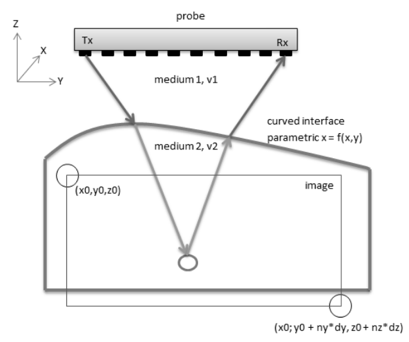
\includegraphics[width=100mm]{surface2.png}
		\caption{Example geometry of the refraction problem}
		\label{fig:cuetfm_geo_descriptor}
\end{figure}

The most basic implementation of TFM has two major drawbacks. The first of these is the fact that the classic TFM algorithm accounts for only one wave propagation speed\cite{holmes_post-processing_2005}. This means that if the wave travels through an interface and reaches a reflector while travelling at a different velocity, the reflector will not appear correctly in the image. This limitation restricts the use of common tools in NDE, such as wedges, in conjunction with TFM imaging.

When imaging, a single sample will be selected from an A-scan for each transmit-receive pair. For a homogeneous material, one can calculate the distance between the element and the point of focus and divide it by the longitudinal velocity of propagation in order to calculate the first arrival of the wavefront at the focal point. For a case where a wave will travel between media the calculation is not so simple as one must account for the change in velocity between the two materials. As the wavefront is somewhat spherical for a typical array configuration, when it refracts through a surface it will do so across a large area as different parts of the wavefront will reach different parts of the surface first. The point at which the wave crosses the surface for the shortest propagation time to the point of interest must be found in order for the wavefront to be treated as a beam to simplify post-processing.

This problem has been well explored and is known as Fermat's principle. The wave that follows this path can be referred to as a ray, as is common in optics\cite{schuster_introduction_1904}. Cassereau et al investigated two ways to approach this problem. One technique, known as the Fermat's Surface (FS) method, calculates delays which are applied to the transmitting elements of an array\cite{cassereau_theoretical_1994}. This method requires recalculation of focal laws for every focal point, and is therefore inefficient. Artefacts are often common in images generated using FS due to abnormally large sidelobes\cite{jones_acoustical_2012}. Time reversal was also investigated. It is an adaptive self-focusing method that requires no a priori knowledge of the propagating medium\cite{cunningham_ultrasonic_2012}.  The time reversal method shows promise but requires transmission of a pulse which is then analysed and used to calculate accurate focal laws for the next transmission. As the aim is to produce a TFM-like image, which will reduce the impact of beam divergence\cite{kitze_saft-reconstruction_2012}, multiple focal points are required. Re-transmission for each focal point is not feasible due to the number that would be required.

An iterative solution to Fermat's principle was presented by Weston et al\cite{weston_time_2012}.  Weston used a curve fitting method to learn the shape of the interface before using an optimisation algorithm to find the point where the ray crosses the interface. The limitation of this approach is the time taken for an iterative solution to be found. 

A virtual array simulating each array element was proposed by Fritsch et al\cite{fritsch_new_2012}. This technique allows rapid computation of focal laws through curved interfaces. Once the positions of the virtual array elements have been determined, the area of inspection can be treated as a single homogeneous medium. The estimated propagation times from the method generally had an error of around 2ns, which would produce sampling errors for an FMC dataset sampled at 100MHz. The maximum sampling frequency of the Phased Array Controllers used to capture experimental data for this thesis is 100MHz. Ideally, the error would be consistently \textless 1ns so that sampling errors would not become statistically relevant.

Tweedy et al applied the techniques described by Brekhovskikh\cite{brekhovskikh_waves_1980} to perform volumetric imaging using the vector total focusing method\cite{zhang_defect_2010}\cite{tweedie_total_2007}. Brekhovskikh focuses on flat layers and only discusses surface waves in curved surfaces. Matuda et al combined a synthetic transmit aperture (STA) with the Sign Coherence Factor method (SCF) to minimise grating lobe noise in images\cite{camacho_phase_2009}. Fermat's standard approach was taken to find the point of refraction\cite{matuda_imaging_2012}.

Another popular solution to Fermat's principle when waves are propagating through a non-homogeneous or anisotropic media is ray tracing. Ray tracing involves quantising the 3D space through which the wave propagates. For each discrete volume, the wave equation is solved so that for each point in time, the position of the wavefront is known\cite{zhang_ray-based_2006}. Jurado et al developed a mathematical model that uses a ghost interface to approximate bending of rays through complex structures\cite{jurado_fast_1998}. The method is based on ray tracing, and the time taken to calculate the path of a single ray is around 1 second. For an ultrasound array configuration scenario, there are multiple sources and multiple receivers each of which would require solving individually. For a 32 element array and a 500 by 500 pixel image, the paths of 8 million rays would need to be calculated. Jurado's method is not feasible at this scale. Ray tracing also provides the positional information of the wavefront at any point in time. For this application, the only knowledge required is the time when the wavefront reaches a point of interest. Another solution that deals with arbitrary interfaces was presented by Sutcliffe et al\cite{sutcliffe_real-time_2012}. They used an iterative minimisation algorithm to pre-calculate wave paths before capturing data to give pseudo real-time imaging. The huge drawback of this approach is the fact that the pre-calculation takes over an hour to complete, rendering it impractical for true real-time imaging applications.

The second limitation of TFM is its computational cost. Consider the start of the imaging process when a full collection of data from every transmit-receive pair of elements (an FMC dataset) is available. In the imaging stage, for each pixel of the image, the following operations have to be performed.  For each transmitter/receiver pair:
\begin{enumerate}[a)]
\item Calculate time of flight of sound along the path between the transmitting element to the pixel and back to the receiving element
\item Accumulate (i.e. sum) the echo value from respective A-scan memory. In the simplest implementation of TFM, one would take each pixel, calculate the times of flight (ToFs) for all combinations of transmit/receive signals, and coherently accumulate respective A-scan samples from the FMC data set. This process results in a large number of loops (for each transmit element, for each receive element, for all x-pixels, for all y-pixels). Both Lambert et al\cite{lambert_performance_2012} and Yiu et al\cite{yiu_gpu-based_2011} have presented papers which use GP-GPU software to generate TFM images. While neither of these papers deal with the problem of refraction, their results will be used as a benchmark for the presented algorithm.
\end{enumerate}

This chapter presents an efficient approach to TFM imaging through an arbitrary interface. Both the imaging methodology and its implementation are novel. Iterative processes are computationally inefficient but they are unavoidable when calculating ray paths through non-flat interfaces. Furthermore, once the intermediary point of the ray path is found, two separate calculations need to take place to find the propagation time from the originating point to the interface, and from the interface to the point of interest within the second material. Considering that this process must be done for each transmit-receive pair for each pixel, there are a large number of calculations to be performed.

It must also be noted that Zhang et al have investigated a similar technique\cite{zhang_efficient_2014} that involves using a smaller dataset then extrapolating this data in order to generate a high-quality image. Zhang proposes generating a sparse grid of known time-of-flights then interpolating to generate a final image. An in-depth study of the errors incurred via this method was performed in order to establish the maximum point separation of the grid before the image quality was affected. 

General Purpose Graphical Processing Units (GP-GPUs) are gaining popularity in the field of ultrasonic imaging due to the number of parallel processes that they can support. While a modern high-end Intel i7 CPU has 4 cores with 8 compute threads, modern NVidia graphics cards contain GPUs with 2880 cores, though only one thread can run on each core. While the CUDA cores are less complex than a CPU core, it is perfectly suited to do simple mathematical operations.

A GPU's main drawback is memory latency; that is the time taken to access a location in memory and deliver its contents to the program. While numerical operations are very fast, fetching stored numbers from memory takes a comparatively long time. Using all of the features available on a GPU, the memory latency can be minimised, thus accelerating the procedure. Another drawback of GPUs is that they do not deal with diverging threads (i.e. processes performing differing operations) particularly efficiently. Cores are clustered in groups of 32, called a warp. Each warp can only perform the same operation per clock cycle, be it reading memory or performing a mathematical operation. If threads on a warp diverge, cores will spend valuable computing time doing nothing waiting for other threads to catch up. It is for this reason that the use conditional statements need to be minimised in parallel GPU computing.

Due to the need to minimise thread divergence, and the fact that the code takes a long time to run regardless of divergence, the iterative solver for Fermat's principle needs to be run as few times as possible. 

While propagation time is not proportional to the depth in the material, it is possible to describe the relationship with a curve. Although it is not known if the coefficients of the curve can be found directly given the parameters of the experiment, it is possible to find a small number of propagation times and from this, calculate a set of coefficients that will describe a depth-time curve for any transmit-receive pair.

The presented method does this, and as such is fast and efficient while retaining the accuracy of non-refractive TFM imaging. This enables an implementation of refractive TFM which is able to produce rapid and accuate results.

\section{Methodology}

TFM imaging is a process which can be referred to as `embarrassingly parallel'. This means that the methodology can be easily split into a number of identical independent processes. With TFM, each pixel and each ToF can be calculated independently, and in parallel at the same time as others, from a single FMC data set. However, as it will be shown later in this work, the order of calculations does matter in terms of computational efficiency. Given a relatively simple set of operations needed for each pixel, GP-GPU computing cards are a good candidate for realisation of the TFM process. With their compute-dense architecture, the memory interface bandwidth becomes the limiting factor in utilising large look up tables. In fact, due to their architecture, some results are faster to be re-calculated on the chip as needed, rather than calculated once and stored\cite{nvidia_cuda_guide}. When considering implementing the TFM process on the GPU, one should consider taking maximum advantage of various subsystems of the GPU architecture. In particular, there are a number of memory subsystems, varying in functionality, bandwidth and latency, and special function units, like texturing units, that can work in parallel with the main streaming processors responsible for the bulk of computation.

The classic way of calculating the time of propagation of a sound ray through a refracting interface is by use of Fermat's principle of shortest time of propagation. To solve this problem, various small-scale optimisation algorithms can be used. Dziewierz described a method for obtaining a computationally efficient, closed-form solution for the equation describing the time of flight of acoustic ray through a 3D planar interface\cite{dziewierz_computationally_2013}. However, the problem now has to be generalized for arbitrary interfaces. Solving this problem for a planar interface comes down to finding roots for a 4th order polynomial equation. It was therefore anticipated that curved interfaces would involve equations such as a 5th order polynomial, or higher. Although there exist methods for finding roots of such equations\cite{wolfram_quintic}, a different approach is used here due to the desire to find a general solution.

The propagation time between neighbouring pixels is a non-linear, but smooth function of space. The approach adopted here approximates the exact solution of the equation that describes propagation delay with an interpolating polynomial. A polynomial was selected as the interpolating function because of the high efficiency with which it can be evaluated on the GPU, and controllable accuracy of the solution, as discussed later in this chapter.


\subsection{Stage 1: Prototype time of flight probing points calculation}\label{sec:phase1}
\begin{enumerate}[a)]
\item The imaging space is divided into straight $z$-lines, as depicted in Figure \ref{fig:cuetfm_geo_zline}\cite{dziewierz_design_2013}, with $z$-coordinates going in a general direction away from the probe. In this implementation, $z$ is the `depth' coordinate related to some arbitrary coordinate system in which the probe elements, refracting surface and TFM image volume is described.

\begin{figure}[htb]
\centering
		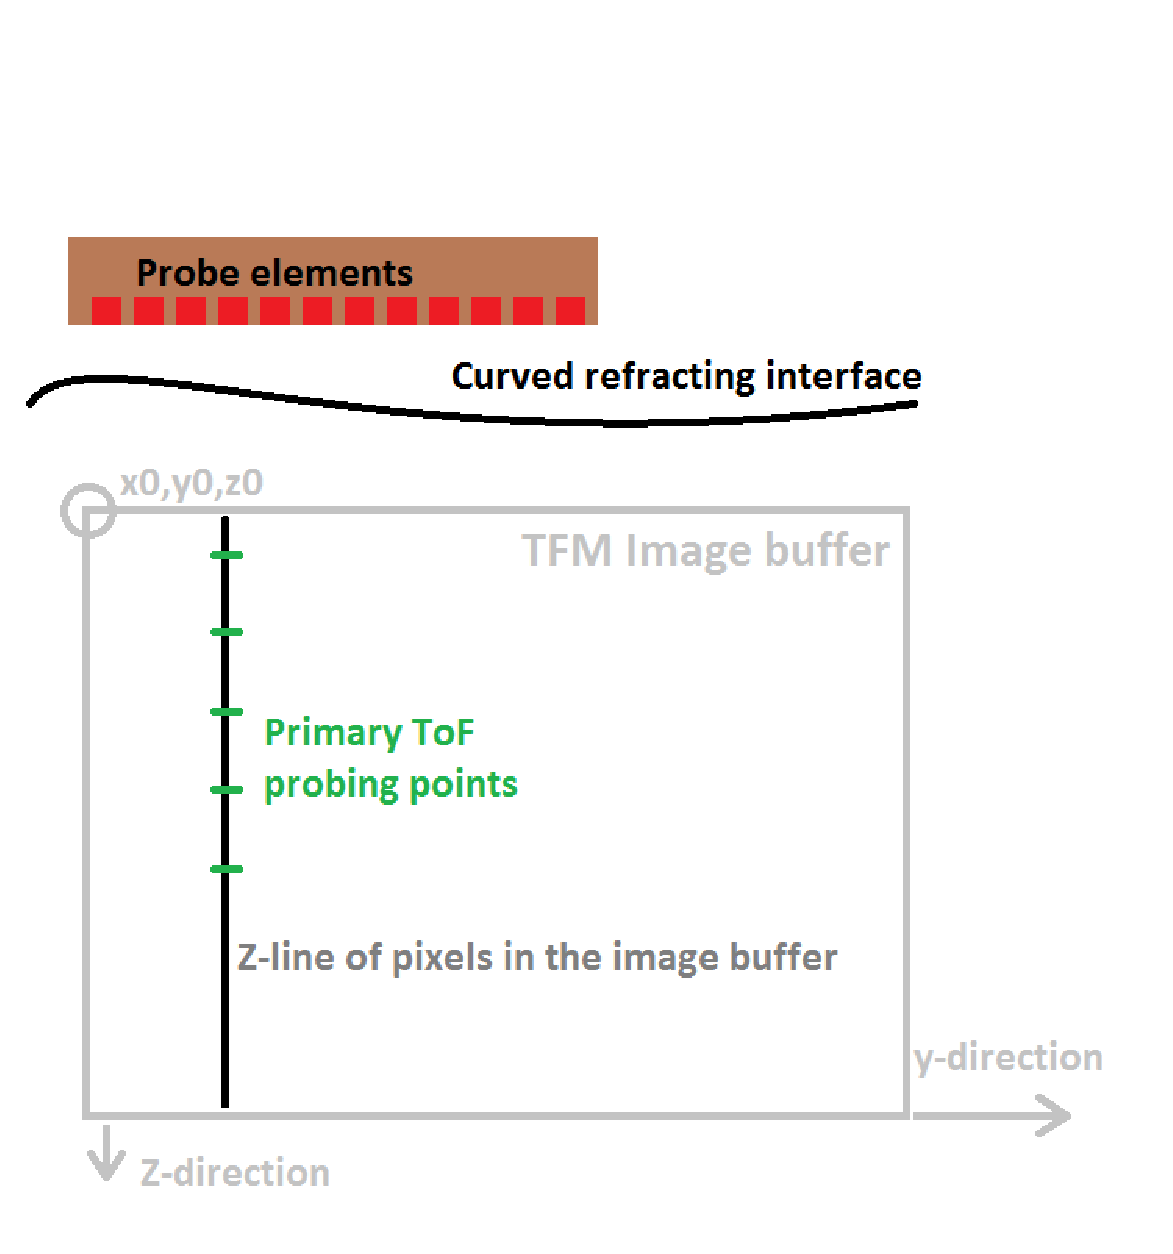
\includegraphics[width=100mm]{zline.eps}
		\caption{Location of probe, refracting material interface, image buffer, and $z$-line of pixels inside the buffer. The linear memory locations progress down-first, then right. The third dimension is $x$.}
		\label{fig:cuetfm_geo_zline}
\end{figure}

\item In order to iteratively find the point of refraction on a surface, the surface must first be defined. Early versions of this process required the surface to be input as a mathematical equation, for example $z = 0$ for a flat surface. A methodology has since been developed that automatically finds the shape of a surface and incorporates this into the solver\cite{mcgilp_inspection_2015}. This methodology involves creating a basic TFM image of the surface and using thresholding to isolate the area where the first reflections occur. It is assumed that coupling takes place through water and that the first large reflection will be that of the material's surface. The estimated surface profile is extracted from the image and input to a curve-fitting algorithm that smooths the result. Finally, the surface is converted to a lookup table and uploaded to the graphics card. Due to the fact that curve-fitting is used on the surface profile, it is expected that this algorithm will not perform well on specimens with a rapidly changing surface profile.

\item For each $z$-line and probe element combination, propagation times for a number of points along the $z$-line are calculated using one of the iterative methods based on Fermat's principle. The number of points was chosen to be 16, and this value remains constant throughout this chapter. Zhang et al explored a similar technique\cite{zhang_efficient_2014}, and investigated the maximum spacing permitted between points before errors were introduced. The Nelder-Mead simplex optimisation method was chosen to find the minima due to its simplicity. Such an algorithm can be optimised for speed. The Newton-Raphson method was also investigated but discounted due to the fact it is prone to converging to local minima. MATLAB (MathWorks, USA) is a technical computing language and IDE. Its inbuilt optimisation function\footnote{\url{www.mathworks.com/help/matlab/ref/fminsearch.html}} is a generalised implementation of the Nelder-Mead method. It was used as basis for a low-level implementation of the methodology that is far more efficient than a general implementation. A number of performance enhancements techniques were used, such as loop unrolling and optimising the code for the desired number of coefficients. This allowed removal of many conditional statements that will impact the speed of the process. This is especially important when porting the code to GP-GPU as the architecture of GPUs does not allow for efficient processing of branches. The spatial distribution of the points can be regular, or generated using affine transformation of Chebyshev nodes as in Equation \ref{eq:Chebyshev} where $n$ is number of points required and $x_k$ is the distance of each point from the origin. These are known as the primary time of flight $= f(z)$ points, where $f(z)$ is some unknown function that describes the time of flight along the $z$-line. 

\begin{equation} \label{eq:Chebyshev}
x_k = \cos \left( \frac{2k - 1}{2n} \pi \right) , k = 1, ... , n 
 \end{equation}



\item The physical time of flight (in seconds) value is scaled to a normalized value that maps into the appropriate fraction of the A-scan, assumed to be coincident with spatial location inside the TFM image buffer.  This single multiplication/offset operation at this point saves thousands of processor cycles that would be needed in Stage 2 to execute the same operation.
\end{enumerate}
\subsection{Stage 2: Pre-calculation of interpolant coefficients}
The primary time of flight data points are divided into two groups. One group is used to fit an interpolating polynomial, and the second group to estimate the error of the approximation to ensure accuracy. This transformation of $f(z)$ samples into interpolating polynomial coefficients is executed using a specialized, non-branching solver as detailed later in this chapter. At this point, the minimal order of polynomial is selected in such way as to fulfil the requirement for accuracy of the approximation, as detailed later in this chapter. The interpolant coefficient database is segmented and optimised for GPUs' on-chip cache, enabling rapid retrieval of the coefficients to the streaming processors.

For a given probe, surface and scene parameter combination, a set of interpolant coefficients can be calculated once and stored for reuse in delay-and-sum imaging. If the probe-refracting surface configuration is changing (for example, when the probe probe is moving over the refracting surface causing the surface profile to change), re-calculation of this database is necessary. This operation is comparatively inexpensive in terms of computing complexity compared to the imaging process. 

\subsection{Stage 3: Delay-and-Sum Imaging}

For most imaging problems, this part of the process is the most computationally expensive, and therefore has been designed to benefit from details of the GPU architecture.

In the GPU, during parallel processing, each thread is made responsible for a single pixel of the image. The thread block size is configured in such way that all the active threads in a block process consecutive pixels from the same Z-line of the image. This allows the threads of the thread block to take a couple of advantages from the GPU's memory architecture, as described below.

For this implementation, a list is employed that describes which A-scans from the FMC buffer will be used in each iteration. This allows use of a single code base to effectively generate images from Sparse Matrix Capture datasets. This table is loaded through the constant cache - also benefiting from the broadcast mechanism, in a similar way to the interpolant coefficient table.

Inside the thread, the outermost and only loop is over the list of A-scans that contribute to a given pixel. For a given A-scan, the thread utilizes the polynomial coefficients obtained in Stage 1 (Section \ref{sec:phase1}) to calculate the respective transmitter-to-pixel and pixel-to-receiver propagation times. 

At this point, one should be aware a particular feature of GPU architecture: shared memory broadcast. The interpolant coefficients corresponding to a single $Z$-line of the final are loaded from device memory into shared memory only once at the beginning of the thread block, and from there, the values are repeatedly broadcast to all threads as needed, using a pointer in memory. This is possible because consecutive A-scans are processed simultaneously across all active threads of the multiprocessor, in lockstep. One could treat this operation as user-managed caching.

The threads evaluate the time of flight using an interpolating polynomial with their respective pixel's coordinate fed into the Horner method\cite{dorn_generalizations_1962}. This operation maps to a short series of very efficient FMA (Fused Multiply Accumulate) instructions with no loop. In effect, the required time of flight value for each pixel is recreated as appropriate. As detailed in Section \ref{sec:phase1}, the resultant value is already scaled such that this value is a pointer that the texturing unit can use to load the appropriate A-scan sample value from the FMC buffer. 

Here another feature of GPU becomes useful to accelerate the retrieval of data. It would normally appear that random memory access is required for the FMC sample retrieval step. However, since all threads evaluate times of flight for a given transmit/receive pair (A-scan) simultaneously, and beginning from the top pixel down, they will request A-scan data that reside at neighbouring and progressing memory locations, albeit with non-integer stride. The texturing units can load requested A-scan data through the L2 cache, which is a high-speed memory unit on the GPU itself. This is very efficient because, typically, an entire A-scan will fit in the L2 cache. In this study an NVidia GTX 580 was used which has approximately 1.5 Megabytes of L2 cache memory. From there, the data block is broadcasted to the texturing units that request it. This way the data is efficiently distributed to the texturing units, which in turn also operate their own, smaller texture cache (depending on the GPU model). The data from L2 cache is reused as many times as there are pixels per $Z$-line, or less, depending on the effect of texturing unit cache.

The texturing units are hardware optimised for this kind of operation as this is essentially the same operation as 3D graphics texturing itself, which a major factor upon which the competitive relative performance between various graphics card models is evaluated. The texturing units select appropriate samples from the A-scan buffer, and provide additional service of interpolation between A-scan samples (super sampling), if necessary, maximising the parallel spread of the computations across the GPU chip. This operation can be referred to as `free' in terms of computational time because as it progresses, the main CUDA cores are executing other threads, preparing a new batch of requests for the texturing units. 

Finally, the threads integrate the A-scan samples they received from the texturing units. At this point, the integration operation can be summation (as in classic TFM) but it can also be a different operation; for example multiplication\cite{lines_rapid_2006} or Phase Coherence Factor calculations\cite{camacho_phase_2009}.

Upon completion of integrating all the A-scans, threads store the computed pixel value in the image buffer, which resides in the global memory. This again is an operation that benefits from the fact that neighbouring threads process neighbouring pixels. The memory write operation is well coalesced and parallel, and fully exploits the main memory bus. Importantly, no synchronisation nor atomic operations are ever needed because by design, no memory write race ever occurs.

Since the image is processed line-by-line, only the interpolant coefficients related to that $z$-line need to be stored in the quickly-accessible on-chip shared memory. For example, for a 128-element probe and interpolating polynomial of maximum order of 7, and single-precision floating point format of the coefficients, $128*7*4 = 4480$ bytes of information are needed to be loaded from global memory per $z$-line, but only once for all threads. Each thread working in this $z$-line re-uses this information using the broadcast mechanism, reading $7*4=28$ bytes of coefficients from this buffer, up to $2*128*128$ times per pixel. This saves a significant amount of time that would otherwise be spent loading data from global memory if the broadcast mechanism was not used\cite{lee_cuda_2012}. 

However, this also means that running more than few blocks of threads per GPU is somewhat counter-productive, as there is a very limited amount of on-chip shared memory available. Therefore this process works best if there are enough pixels in the $z$-line, and not many $z$-lines processed in parallel. For images with a small number of pixels in the $z$-direction the GPU can potentially be under-utilised. This is due to the fact that there are a number CUDA cores on a GPU and multi-threading will not take place by default. If there are fewer $z$-pixels than the number of CUDA cores, these cores will remain idle during the computation process. 

Incidentally, it is of practical benefit to have the highest image resolution along the depth axis ($z$-line), because in such cases the constructive/destructive interference between A-scans produces the best TFM process gain (contrast improvement) and phase accuracy. If fewer than 7 pixels per wavelength resolution are used, the TFM process may not achieve its peak process gain due to sampling phase error\cite{wagdy_errors_1985}. The same applies to other TFM-like algorithms like Phase Correlation Factor algorithm.

Overall, the process described is extremely efficient and takes approximately 48 hardware cycles per integrated A-scan (this measured value includes all exposed latencies) per pixel, and is the main source of performance of our implementation.

\subsection{The non-branching polynomial interpolant coefficient solver}
In order to find the coefficients for interpolants needed for this imaging algorithm, a well-known least-square method of fitting a polynomial into a set of points by solving a matrix-quadratic equation can be used. 

Typical CPU implementations of this method utilize loops and conditional jumps to allow single implementations of a code to solve for an arbitrary order of polynomial and arbitrary number of data points, sometimes even reordering the data first to minimize the numerical errors. However, in this case, the speed of execution of the solver being of utmost importance, it was decided to compile a range of specialized solvers, each taking exclusively a fixed number of data points and returning a fixed order of polynomial. This approach allows a linear, non-branching code for each case to be obtained. A subset of statistics on the addition and multiplication operation count versus number of inputs and polynomial order has been gathered in Table \ref{table:cuetfm_poly_operations}.

\begin{table}[htbp!]
\begin{center}
	\begin{tabular}{| p{2.4cm} | p{2cm} | p{1.8cm} | p{1.8cm} | p{2cm} | p{1.6cm} |}
	\hline 
	\textbf{Polynomial order} & \textbf{Number of input points} & \textbf{FMA ops count} & \textbf{MUL ops count} & \textbf{ADD + SUB ops count} & \textbf{Total op count} \\ \hline \hline 
	4	& 6 & 120 & 182 & 44+35 & 381 \\ \hline
	4	& 10 & 192 & 260 & 76+36 & 564 \\ \hline
	5	& 8 & 330 & 445 & 76+99 & 950 \\ \hline
	5	& 12 & 453 & 571 & 116+98 & 1238 \\ \hline
	6	& 10 & 743 & 976 & 119+296 & 2134 \\ \hline
	6	& 14 & 935 & 1152 & 167+296 & 2550 \\ \hline
	\end{tabular}
	\caption{Computational operations required to compute polynomials}
	\label{table:cuetfm_poly_operations}
	\end{center}
	\end{table}

Table \ref{table:cuetfm_poly_operations} shows statistics of computation cost for calculating the interpolating polynomial coefficient as a function of polynomial order and number of contributing data points. Each version of the algorithm also requires a single reciprocal operation.

The code has been obtained using Wolfram Mathematica Computer Algebra System, using a method similar to the one Dall'Osso described in detail in Computer algebra systems as mathematical optimizing compilers\cite{dallosso_computer_2006}. 

The code obtained only requires multiply-accumulate operations and a single reciprocal, and uses no jumps or conditional statements whatsoever. The benefit of such an approach is that such code will execute efficiently on a GPU, solving multiple $z$-lines in parallel. It is appreciated that such approach is not well suited for poorly conditioned inputs, and will allow the numerical errors to surface in the results, even when using double precision arithmetic. However, as argued in the next section, in this application, the inputs are always well conditioned and the observed numerical errors are acceptable. 

\section{Results}
\subsection{Selection of polynomial order and error analysis}
In order to establish confidence in the proposed method, it is necessary to perform a detailed error analysis of the algorithm. The calculated time of flight errors come primarily from 3 sources:
\begin{enumerate}[a)]
\item Inaccurate primary time of flight solver;
\item Inherent method inaccuracy of polynomial approximation;
\item Numerical inaccuracy of polynomial coefficient solver. 
\end{enumerate}
In this work, it is assumed that a) is exact; errors incurred by the primary time of flight solver have been reduced to the point where they negligible. Any additional error added may be caused by the way computers handle floating point numbers. Accounting for this eventuality is considered out of the scope of this thesis. Here only b) and c) are considered as source of errors.

To estimate the end-to-end time of flight calculation error of this process, the following method has been applied:
\begin{enumerate}[1)]
\item Prepare a set of pre-calculated times of flight for a typical imaging scenario; 
\item Convert the subset of pre-calculated times of flight to interpolant coefficients, and then back into full grid of times of flight; 
\item Calculate the peak difference between original and processed time of flight data. 
\end{enumerate}

The summary of results for the imaging scenario depicted in Figure \ref{fig:cuetfm_geo_zline} is gathered in Figure \ref{fig:cuetfm_peak_error} and are shown as a function of the polynomial order used.  

\begin{figure}[htb]
\centering
		\includegraphics[width=100mm]{peak_error.eps}
		\caption{Mean and peak time of flight calculation errors resulting from using a polynomial of a given order as interpolant for a given imaging scenario.}
		\label{fig:cuetfm_peak_error}
\end{figure}


The proposed direct no-branch solver returns values that are close enough to the results of MATLAB's QR solver to be considered negligible. This holds true up to an interpolant order of 5. If a higher order interpolant is needed, the QR solver is recommended.

The significance of these results are as follows. For a source signal sampling of 50MHz, the useful bandwidth of the sampled signal is considered no better than approximately 17MHz;  full sine wave cycle at that frequency is $58.8\e{-9}$ seconds long; therefore to obtain phase accuracy better than 1/4 cycle (worst case scenario), the error must be less than 1.47\e{-8} seconds. From Figure \ref{fig:cuetfm_peak_error}, it can be observed that a polynomial order of 5 or higher must be selected for interpolation. In this case, the phase accuracy for a 5MHz signal will be better than 1/15 cycle. 

Note that the cited timing errors are peak errors and the average timing error will be much lower. In any case, it is possible to obtain an arbitrarily low peak error estimate by raising the interpolant order (up to the limit of numerical representation accuracy). This will be at the cost of a minor decrease in Stage 2 performance. 

It is appreciated that the evaluation method presented here does not give strict upper bound for error; however, it can be easily repeated for any practical imaging scenario and the minimum required order calculated for a specific imaging scenario.

\subsection{Implementation benchmark}
The proposed process consists of several stages that can be executed independently, and thus, benchmarked independently. In other publications, the overall performance in practical scenario is typically expressed in frames per second for a given specific scenario\cite{choe_gpu-based_2013,phuong_design_2015,gjerald_real-time_2011}; here a more synthetic approach is taken. Each stage is benchmarked independently and then combined to estimate overall performance for a given set of input parameters. These results are shown in Table \ref{table:cuetfm_resuls}.

\begin{table}[htbp!]
\begin{center}
\begin{tabular}{|p{2.5mm}|p{40mm}|p{30mm}|l|p{25mm}|l|}\hline
  & \textbf{Stage Name} & \textbf{Options} & \textbf{Platform} & \textbf{Performance Unit} & \textbf{Result} \\ \hline\hline
	1 & Stage 1: Calculating prototype Time of Flight points & Planar interface z=0 & GPU & Points/second $\times 10^6$ & 77.9 \\ \hline\hline
	2 & \multirow{4}{*}{\parbox{40mm}{Stage 2: Transform from time points set into interpolant coefficients}} & 8 points into 5th order, fast solver & GPU & \multirow{2}{*}{\parbox{25mm}{Lines/second $\times 10^3$}} & 23 538 \\ \cline{1-1} \cline{3-4} \cline{6-6}
  3 & & 8 points into 5th order, fast solver & CPU & & 2 960 \\ \cline{1-1} \cline{3-4} \cline{6-6}
	4 & & 8 points into 5th order, QR solver & CPU & & 70 \\ \cline{1-1} \cline{3-4} \cline{6-6}
	5 & & Double precision, 14 points into 7th order, QR solver & CPU & & 68.5 \\ \hline\hline
	6 & Stage 3: TFM integration & Nearest sample interpolation & GPU & Paths/second $\times 10^9$ & 26.7 \\ \cline{1-6}
\end{tabular}
\caption{Results of benchmarking for each stage}
	\label{table:cuetfm_resuls}
	\end{center}
	\end{table}

For each stage of the process, an appropriate measure of performance is introduced. For finding the initial times of flight, the metric is time of flight points calculated per second; for calculating the polynomials, it is lines per second (as each atomic transform deals with entire image line); for creating the final image, paths per second are used - as each atomic operation deals with estimating time of flight over a specific path. 

With such metrics, one can trade number of pixels, number of probe elements, and the Tx/Rx firing scheme against the performance of the particular GPU system used and frame rate achieved. For any TFM image resolution and number of elements of the probe, the total calculation cost can be obtained. For example, for an image with $1024^{2}$ pixels, and 64-element probe operating in full FMC firing scheme, the computational cost of the TFM method is $2*1024^{2}*64^{2} = 8.6\e{9}$ paths. 

In the example above, assuming that a polynomial order of 5 is selected, with 8 sampling points, there are $8*1024*64 = 524\e{3}$ primary times of flight to be calculated initially, and $1024*64= 65.5\e{3}$ interpolant coefficient sets to be obtained in the second stage. To create an image from this data, for each pixel, Tx-to-pixel time of flight is calculated once and then for each of these, pixel-to-Rx is calculated, resulting in $1024^2*64^2 = 4.3\e{9}$ paths. The symmetry of the time of flight in the FMC is exploited, halving the actual times of flight combination count. Assuming that the FMC data is uploaded to the GPU asynchronously, each frame will take 0.2 sec to compute; image generation takes 82\% of the total time. Therefore any future improvement has to be concentrated in this stage of the process. One obvious improvement would be to introduce partial on-chip caching of the calculated times of flight; this option offers potential for future research. The performances cited in this chapter scale almost linearly over multiple GPUs, for example, processing times are approximately halved when comparing an NVidia GTX 580 to an NVidia GTX590, which has two of the GPUs used in the former. This comparison is not intended to highlight the differences between hardware platforms, but to show the effects of algorithm choice (see rows 3 and 4 of Table \ref{table:cuetfm_resuls}).

\subsection{Experimental validation}

\subsubsection{Cylindrical Surface}

The experimental setup is shown in Figure \ref{fig:cuetfm_experiment_setup}. The probe is a 128-element, 5MHz, linear phased array probe (Vermon, France), and the Phased Array Controller is a Dynaray (Zetec, USA). The probe is placed over a half-cylinder of solid PVC material, in which a flat bottom hole has been drilled out. In this process, the location and shape of the surface have already been measured and input to the imaging algorithm.

The algorithm returns the expected image; the reflection coming from the hole is blurred out when the refraction is not taken into account (Figure \ref{fig:cuetfm_experiment_uncorrected}). When the refracting surface is taken into account (Figure \ref{fig:cuetfm_experiment_corrected}), the reflection is properly located and focused and the amplitude of the feature is increased by 4.57dB. The large black patches on the sides of the cylinder reflection are side lobes, as expected for this probe type and experimental configuration. Figure \ref{fig:res4} shows the refracted TFM result in Figure \ref{fig:cuetfm_experiment_corrected} with a higher dynamic range.

\begin{figure}[htbp!]
\centering
		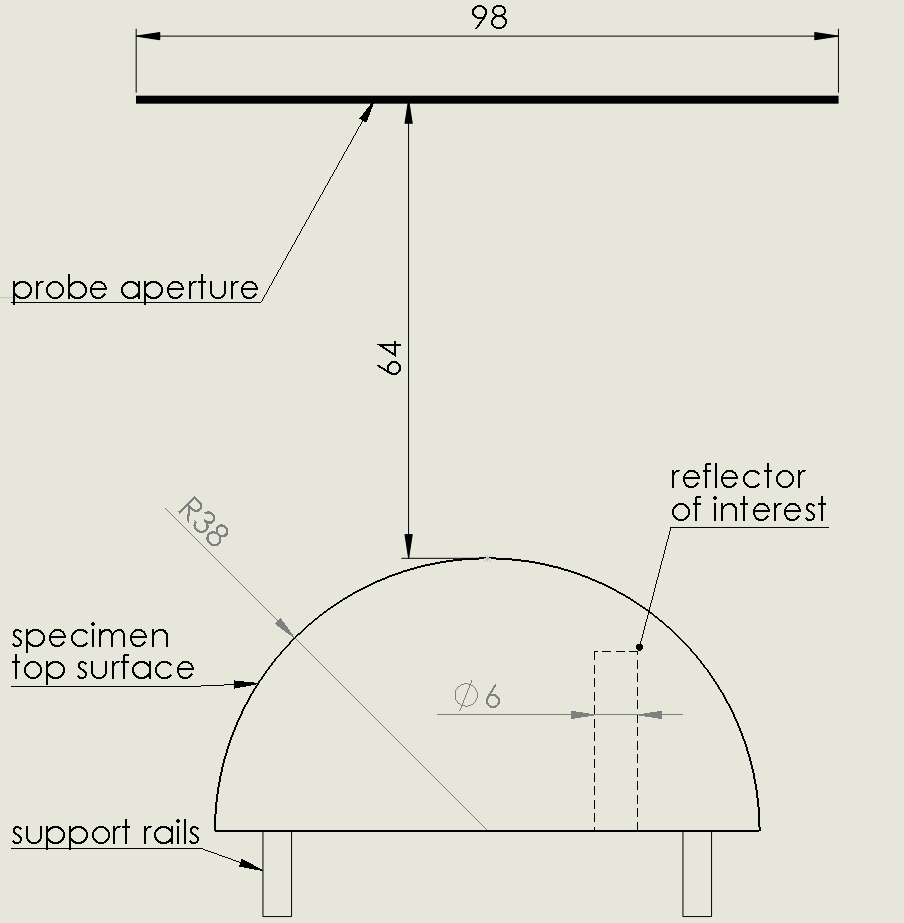
\includegraphics[width=125mm]{schematic.png}
		\caption{Schematic drawing of the PVC specimen submerged in water, and aperture of the 128-element 5MHz linear array. All dimensions are in mm.}
		\label{fig:cuetfm_experiment_setup}
\end{figure}

\begin{figure}[htbp!]
\centering
		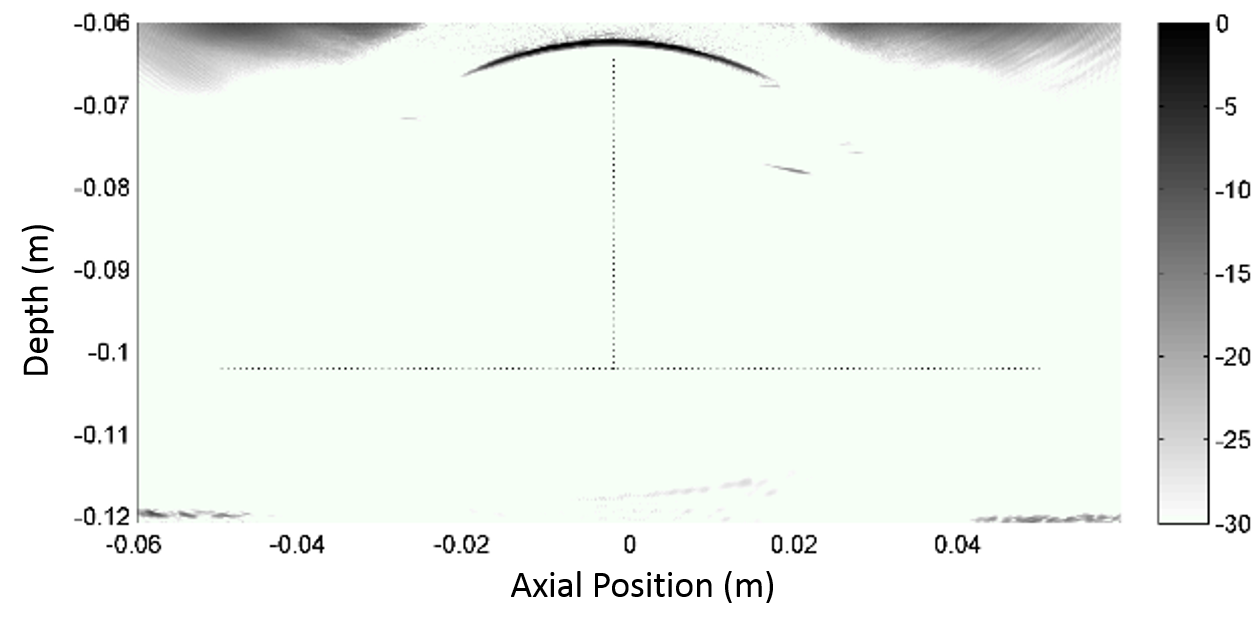
\includegraphics[width=\textwidth]{result-uncorrected.png}
		\caption{The image of the flat bottom hole inside the specimen - no refraction applied. Guides are shown in the image to illustrate the centre and bottom of the semi-cylinder}
		\label{fig:cuetfm_experiment_uncorrected}
\end{figure}

\begin{figure}[htbp!]
\centering
		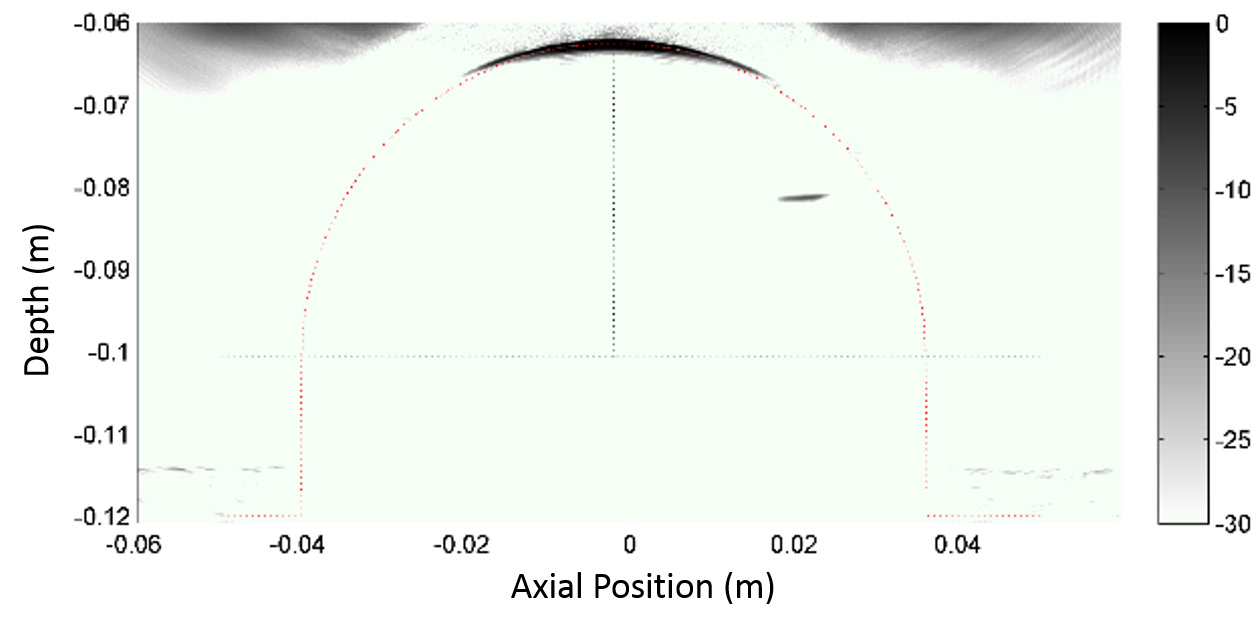
\includegraphics[width=\textwidth]{result-corrected.png}
		\caption{The image of the reflector as in Figure{~\ref{fig:cuetfm_experiment_uncorrected}}, but with correct refracting surface taken into account. The amplitude of the reflector is 4.57dB higher and the reflector is correctly positioned and flat. The overlay depicting the centre and bottom of the semi-cylinder sample are also shown in this image.}
		\label{fig:cuetfm_experiment_corrected}
\end{figure}

\begin{figure}[htbp!]
\centering
		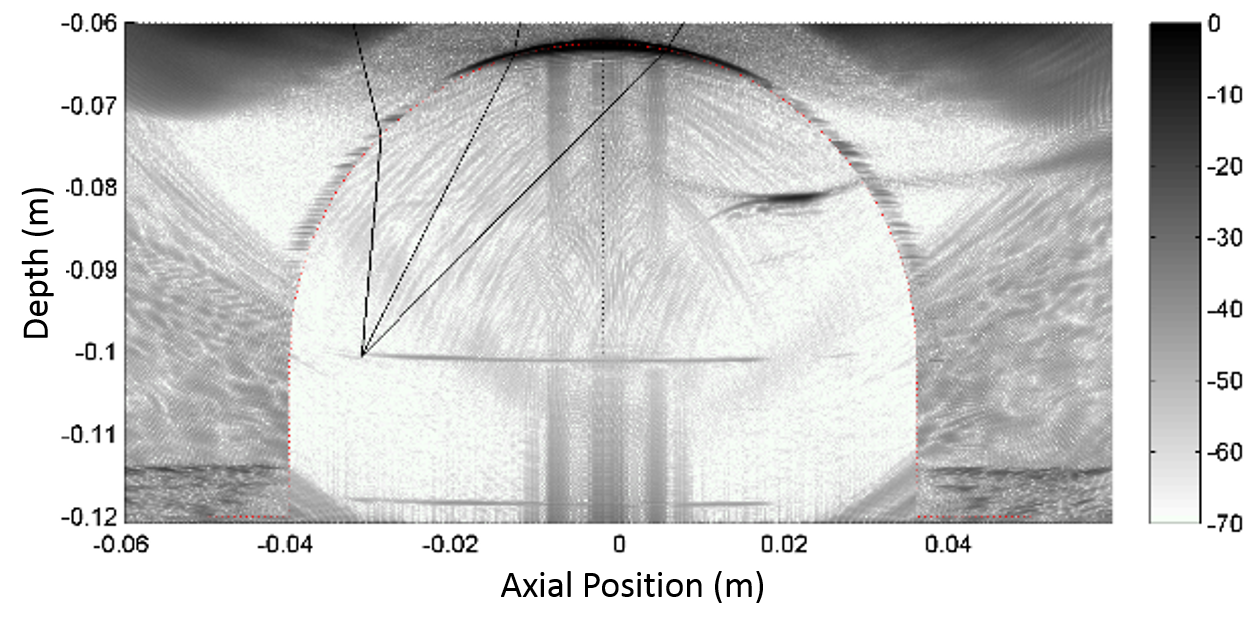
\includegraphics[width=\textwidth]{result-highdr.png}
		\caption{The corrected image with a high dynamic range. The correctly flat back wall is visible at -42dB from the top surface. The 3 black straight lines exemplify calculated ray paths between the 3 of the probe elements and a pixel in the image.}
		\label{fig:res4}
\end{figure}
\clearpage
\subsubsection{Machined Block}\label{sec:ail_result}

The surface of a stainless steel block was machined in order to create a surface through which inspection would be challenging. A photograph of the block is shown in Figure \ref{fig:ailidh1}. The area that is to be imaged is highlighted in the figure via a blue rectangle. The experiments using this block did not use a pre-input surface profile and instead relied on the software being capable of recognising and accounting for the surface automatically\cite{mcgilp_inspection_2015}. All experiments using this block used a Dynaray (Zetec, USA) phased array controller and a 128 element linear 5 MHz array (Vermon, France).

\begin{figure}[htbp!]
\centering
		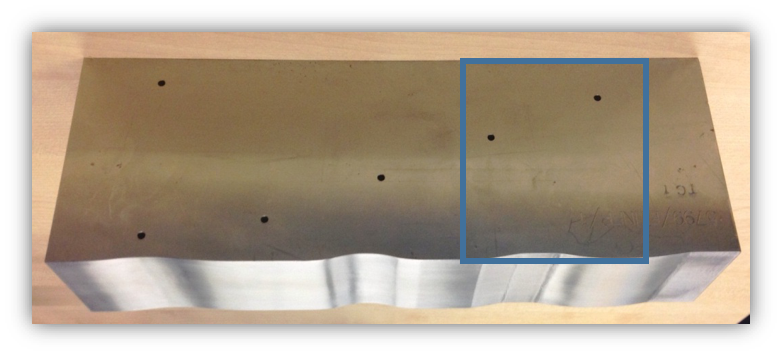
\includegraphics[width=75mm]{ailidh1-new.png}
		\caption{A machined stainless steel 316L block, showing the area to be imaged. The array was placed on a wedge coupled to the top of the block, relative to the image.}
		\label{fig:ailidh1}
\end{figure}

The block was initially tested from the underside. This was to present a simple scenario to test the surface recognition algorithm before inspecting the specimen through the complex surface. A probe was placed on a 14.5$^\circ$ wedge and Full Matrix Capture data recorded.

\begin{figure}[htbp!]
\centering
		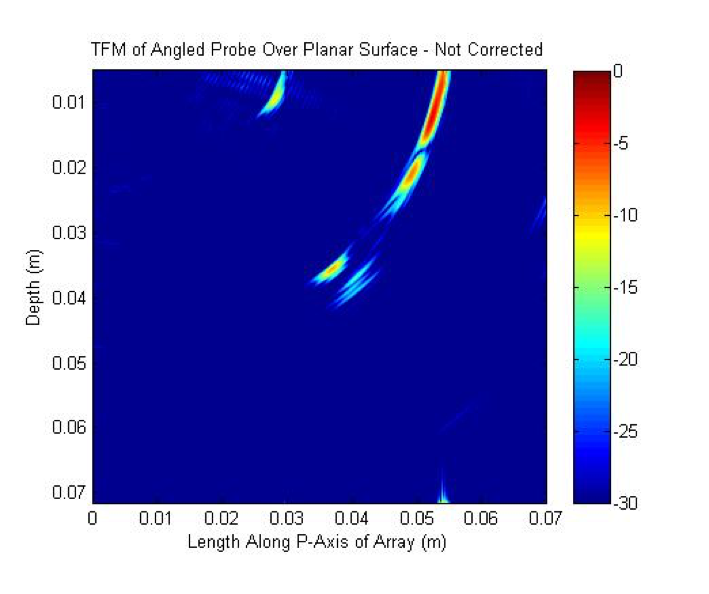
\includegraphics[width=100mm]{ailidh4.png}
		\caption{TFM after incorrect planar refraction}
		\label{fig:ailidh4}

		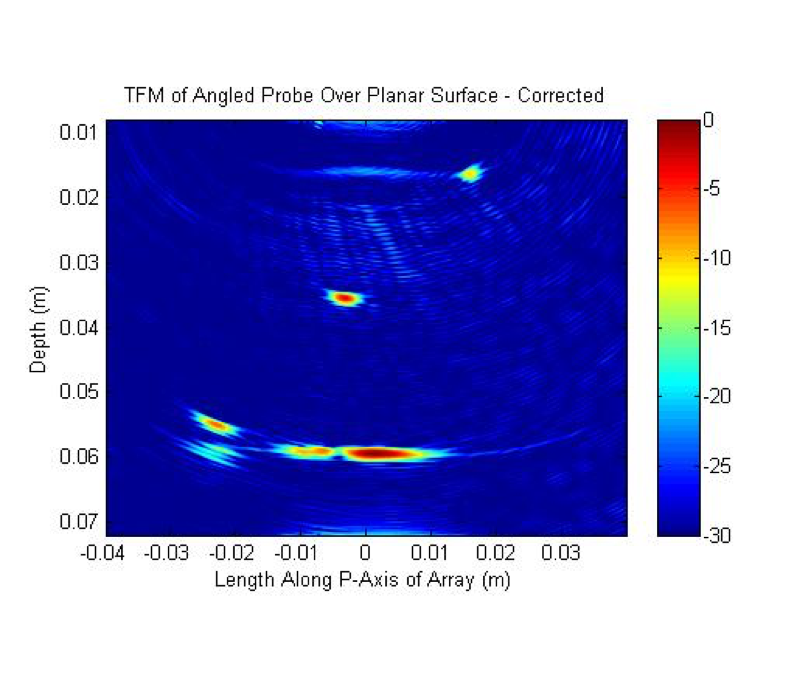
\includegraphics[width=100mm]{ailidh5.png}
		\caption{TFM after corrected planar refraction}
		\label{fig:ailidh5}
\end{figure}

Figures \ref{fig:ailidh4} and \ref{fig:ailidh5} show the uncorrected and corrected TFM images respectively. The automatic surface correction was found to work well with planar surfaces, as the back wall became visible in the correct position at a depth of 60mm and the side drilled holes can also been seen in the image.

An array was then fixed to a stand, and the block inspected from the machined side via water coupling. The area of the block inspected is shown in Figure \ref{fig:ailidh6}.

\begin{figure}[htbp!]
\centering
		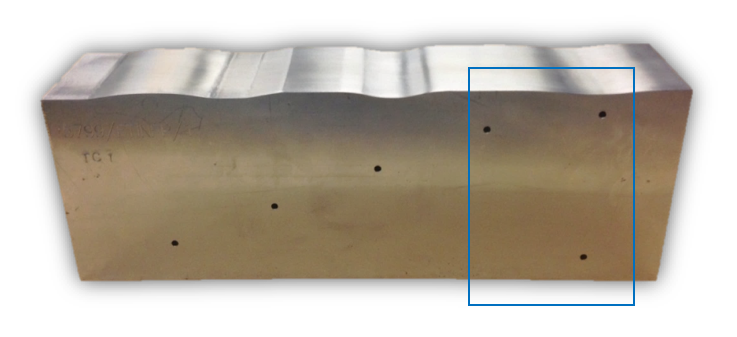
\includegraphics[width=75mm]{ailidh6.png}
		\caption{The area of the machined block to be inspected}
		\label{fig:ailidh6}
\end{figure}

The output of the surface recognition algorithm was checked to ensure that the surface was being correctly identified. The surface profile is shown overlaid on the TFM image of the surface in Figure \ref{fig:ailidh7}. It can be observed from the image that the programmatically identified surface conforms well to the surface seen in the experimental image. McGilp has performed additional research into the accuracy of the surface recognition algorithm, but this is considered out of scope for this body of work\cite{mcgilp_adaptation_2016}.

\begin{figure}[htbp!]
\centering
		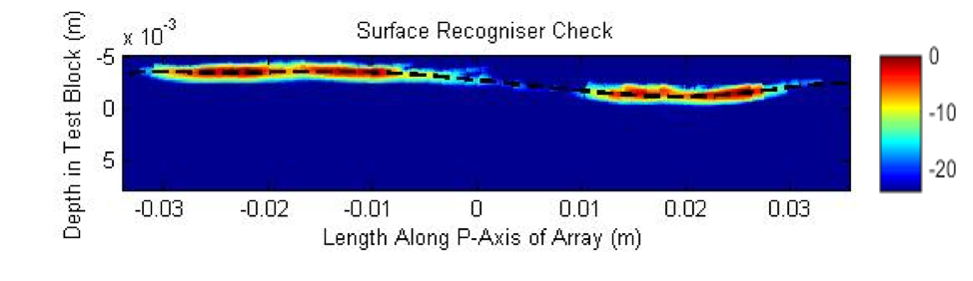
\includegraphics[width=\textwidth]{ailidh7_bar.png}
		\caption{The surface profile of the machined block, shown with dB compression}
		\label{fig:ailidh7}
\end{figure}

Finally, the Total Focusing Method is applied to the FMC dataset. The resulting image is shown in Figure \ref{fig:ailidh8} and with a dynamic range of 20dB. The dynamic range has been shifted to maximise the reflections from the side-drilled holes.

\begin{figure}[htbp!]
\centering
		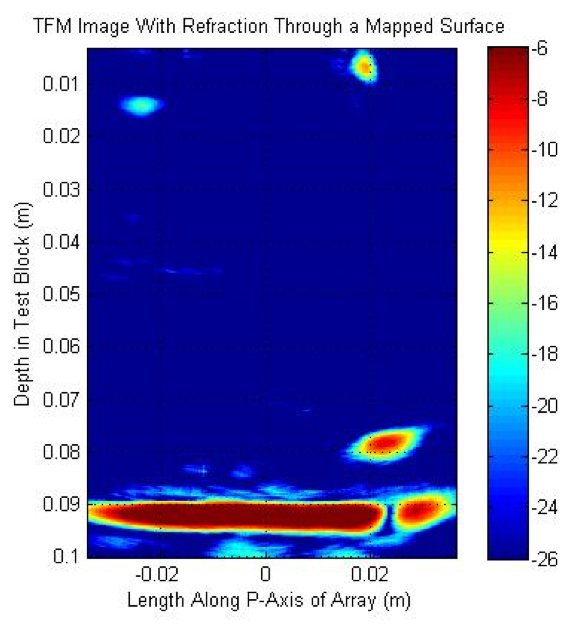
\includegraphics[width=100mm]{ailidh8.png}
		\caption{The corrected TFM image of the area shown in Figure \ref{fig:ailidh6}}
		\label{fig:ailidh8}
\end{figure}

The three side-drilled holes can be seen clearly in Figure \ref{fig:ailidh8} and in the expected locations. From this image, the conclusion can be drawn that the automatic surface recognition algorithm works well, alongside the TFM algorithm that has been designed to cope with an arbitrary surface.

To further ensure that the results are accurate datasets were captured from across the entire sample, processed, and the results stitched together to form an image of the complete block. The results of this are shown in Figure \ref{fig:ailidh9}.

\begin{figure}[htbp!]
\centering
		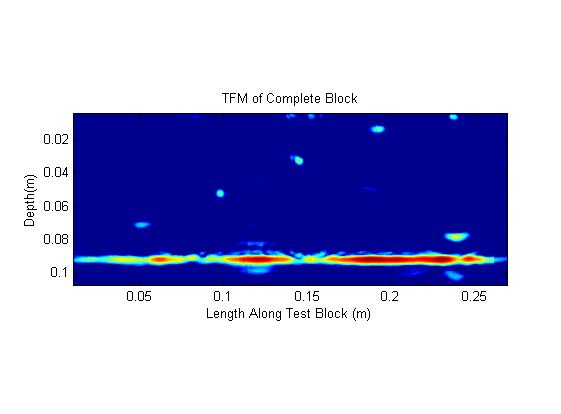
\includegraphics[width=\textwidth]{CompleteBlock.jpg}
		\caption{The corrected TFM image of the entire block}
		\label{fig:ailidh9}
\end{figure}

\section{Discussion}

The solution described in this chapter can be viewed as a way of lossy data compression, where a time of flight look-up table is replaced with a function taking from a limited set of data, to reconstruct parts of the content of the original look-up table when and where needed. The efficiency of this solution comes from transforming the time of flight calculation problem in a way that maps well to the hardware resources that are available in GPU processors. Due to the speed of modern processors compared to the memory transfer speed, it is computationally more efficient to regenerate the data from a `compressed' version than to transfer the excess data to GPU memory and spend time accessing it.

This chapter demonstrates that advanced imaging algorithms that were previously considered to be of research interest only, or limited to military or nuclear applications only due to their cost, can be currently implemented in affordable consumer grade hardware.

This work also allows the possibility of bringing advanced ultrasonic imaging to automated applications where classic phased array imaging is currently prevalent. The aerospace industry routinely conducts non-destructive testing using wheel probes to couple an array to a component as a robot co-ordinates with a phased array controller for acquisition. The wheel is deformable and will therefore change shape as the coupling pressure alters throughout the course of a scan. This is a problem easily solved with conventional phased array but presents a problem when varying focal laws are required to perform TFM or similar imaging algorithms. The use of the presented methodology allows real time TFM imaging in inspection scenarios like this.


% ------------------------------------------------------------------------


%%% Local Variables: 
%%% mode: latex
%%% TeX-master: "../thesis"
%%% End: 
